% !TEX TS-program = pdflatex
% !TEX root = ../tesi.tex

%************************************************
\chapter{Strumenti Aumentati}
\label{chp:strumentiaumentati}
%************************************************

Lo strumento aumentato è una pratica che consente ad uno strumento musicale
tradizionale di esprimere sonorità inesplorabili al solo livello fisico. Allo
strumento tradizionale vengono così aggiunti uno più elementi elettroacustici
estranei allo strumento stesso. A volte a questa \emph{aumentazione} si
accompagna anche l’aggiunta nello strumento di uno o più oggetti. Le sonorità
riescono ad esprimere una qualità di timbri, durate e altezze in numero
estremamente superiore a quelle riscontrabili nell’uso tradizionale degli
strumenti.

Sono diversi gli strumenti che possono essere aumentati, ne viene qui fatta una
breve panoramica prendendo in esame un pianoforte, degli strumenti a percussione,
un clarinetto, un sassofono ed un flauto.

\begin{figure}%[t!]
\centering
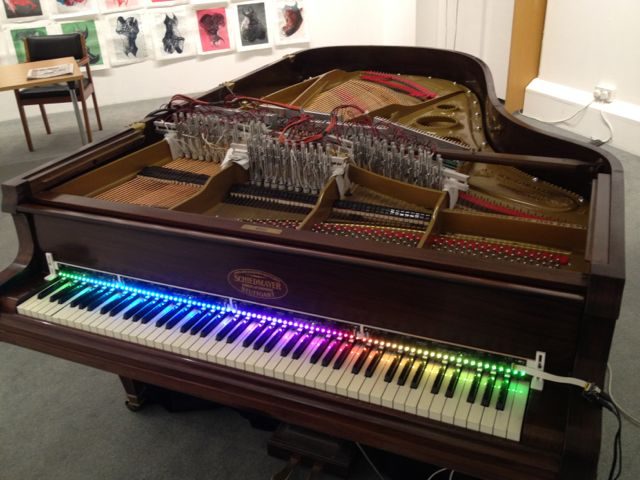
\includegraphics[width=0.99\columnwidth]{Graphics/foto/mrp-aberystwyth.jpg}
\caption[]{Magnetic Resonator Piano.\\ Electromagnetically augmented grand piano}
\label{mrp}
\end{figure}

\section{MRP (Magnetic Resonantor Piano)}

Lo strumento \emph{MRP} è un pianoforte ideato da Andrew McPherson dotato di
elettromagneti  che inducono direttamente vibrazioni nelle corde del pianoforte, generando vibrazioni acustiche indipendentemente dai martelletti, senza la
necessità di amplificazione esterna.

Si generano così \emph{sustain} infiniti, variazione di intonazione e nuovi
timbri, il tutto controllato dalla tastiera del pianoforte. L'\emph{MRP} è
stato inizialmente progettato come un'estensione del pianoforte, consentendo
al pianista di modellare continuamente ogni nota in termini di dinamica,
intonazione e timbro, pur mantenendo la ricchezza e le sfumature del pianoforte
a coda acustico.

L'\emph{MRP} è in grado di fornire sonorità diverse da quelle del pianoforte
tradizionale infatti quando i tasti vengono premuti delicatamente gli
elettromagneti producono molte delle qualità acustiche del pianoforte
escludendo la sonorità del colpo del martelletto. Utilizza 88 attuatori elettromagnetici per coprire l'intera gamma del pianoforte. Quando un singolo
magnete è attivo la relativa corda, o il gruppo di corde, di acciaio viene
tirata verso l’alto e di conseguenza quando la corrente viene interrotta la
corda ritorna nella posizione originale. Modulando la corrente alla frequenza
della corda o ad un suo armonico, la corda viene fatta vibrare senza essere mai
stata colpita dal martello. I segnali audio per gli elettromagneti provengono
infine da un computer,controllato dalle azioni dell’esecutore sulla tastiera.
È possibile un'ampia gamma dinamica che comprende anche toni appena superiori
al silenzio. Sulla tastiera del pianoforte è posizionata una barra scanner
ottica personalizzata che registra l'angolo continuo di ciascun tasto e manda
il segnale al computer\footnote{Andrew Mcpherson, \emph{The magnetic resonator
piano brings continuous note shaping to the acoustic piano}.
\url{https://instrumentslab.org/research/mrp.html}}.

\begin{figure}%[t!]
\centering
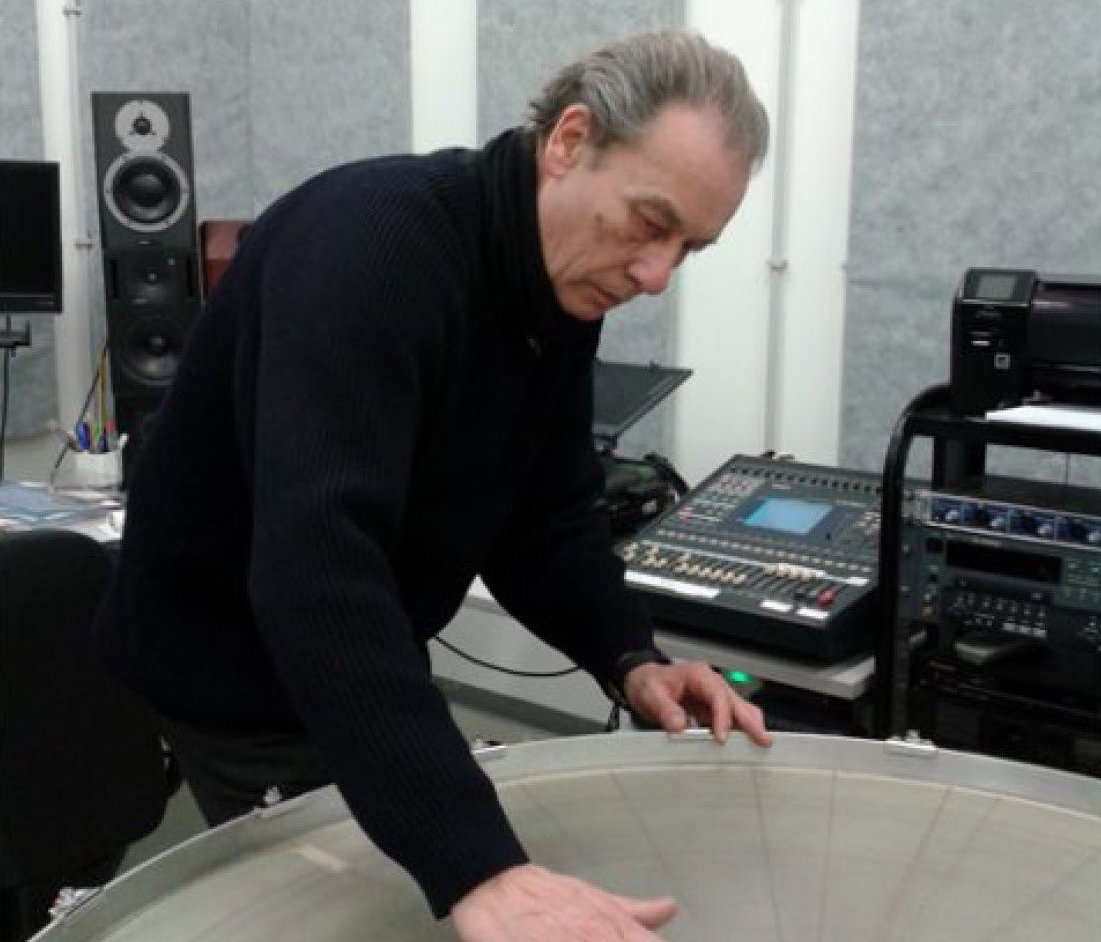
\includegraphics[width=0.99\columnwidth]{Graphics/foto/michelangelo_lupone_recadre}
\caption[]{Michelangelo Lupone.\emph{Feed-drum}.}
\label{mrp}
\end{figure}

\section{Feed-drum}

Il \emph{feed-}drum, nasce in seguito ad in lavoro musicale e scientifico
intorno all’opera \emph{Gran Cassa} (1999) di Michelangelo Lupone.

\begin{quote}
La grancassa sinfonica, lo strumento a percussione più grave, è stata introdotta
nell’orchestra solo nel XVIII secolo e nel secolo successivo ha raggiunto la
forma che oggi conosciamo.

In particolare la forma che era stretta e lunga, com’è rimasta nelle bande
militari, è stata portata a 80-90 cm di diametro e 35- 50 cm di fusto; questo
è chiuso da uno o da ambedue i lati con membrane di pelle naturale tenute in
diversi modi da sistemi che provvedono a regolarne anche la tensione.
La versione più grande, adeguata ai massimi organici orchestrali, è chiamata
grancassa imperiale, ha due membrane e raggiunge 102 cm di diametro. [\ldots]
L’utilizzo della grancassa, per quanto sostanziale in orchestra e costante da
Mozart in poi, è considerato secondario e ristretto a pochi modi di emissione
del suono: il rullo (nota lunga), spesso finalizzato al crescendo, il colpo di
riempimento 4 nelle sequenze ritmiche.

Non sono studiate tecniche specifiche, come nel caso dei timpani, e i battenti
tipici sono la mazza e le bacchette da timpano. L’idea di un’opera musicale,
interamente basata su questo strumento, è nata dall’osservazione dei modi
vibrazionali della membrana.
\end{quote}

Questo strumento fu costruito con lo scopo di studiare i comportamenti di una
membrana sottoposta a una sollecitazione impulsiva, isolando i modi armonici.

\begin{quote}
Le sperimentazioni sono state fatte con l’intento di raggiungere i seguenti
obiettivi:

\begin{enumerate}
  \item variazione della frequenza di base attraverso l’introduzione di vincoli
nodali posti sulla membrana,
  \item distinzione di più timbri in base al tipo, al modo e alla posizione
dell’eccitazione,
  \item modulazione del suono attraverso glissandi, vibrati, portamenti e
micro-articolazione ritmica,
  \item variazioni continue e a gradini della dinamica, in base al tipo di
  smorzamento imposto alla membrana.
\end{enumerate}

\end{quote}

Sulla grancassa fu applicato un microfono a contatto collegato ad un altoparlante
posizionato sotto la membrana.
L’altoparlante ha un diametro di 18 pollici ed é posizionato ad una distanza di
11 cm dalla membrana superiore.

La presenza della seconda pelle della gran cassa , oscillando a fase diverse
dalla principale, non permetteva di tenere l’intonazione della fondamentale di
$30Hz$ e per questo venne rimossa.

Inoltre il corpo con i tiranti della gran cassa fu appositamente costruito da un
artigiano in metallo per mantenere meglio l’accordatura.

Per lo stresso motivo per la membrana fu adottato  un materiale sintetico in
quanto una vera pelle sarebbe stata più soggetta a deformazioni con il tempo.
Il sistema così ideato riesce ad innescare un processo di feedback, tale da far
oscillare la membrana in modo tale che il suono ha una durata tendente
all’infinito.

L’interprete ha a disposizione un pedale di espressione con cui controlla
l’intensità del feedback.

\begin{quote}
Lo smorzamento della membrana e il conseguente decadimento del suono, si possono
regolare, così da isolare i modi alti di vibrazione con l’azione combinata dei
nodi posti sulla membrana dall’esecutore tramite le mani e della quantità di
energia immessa nel feedback. La sperimentazione del sistema ha permesso di
individuare e di segnare sulla superficie della membrana una mappa semplificata
dei modi oscillatori basata sulle fusioni di Bessel composta da 13 diametri e
8 cerchi nodali
\end{quote}

\begin{figure}%[t!]
\centering
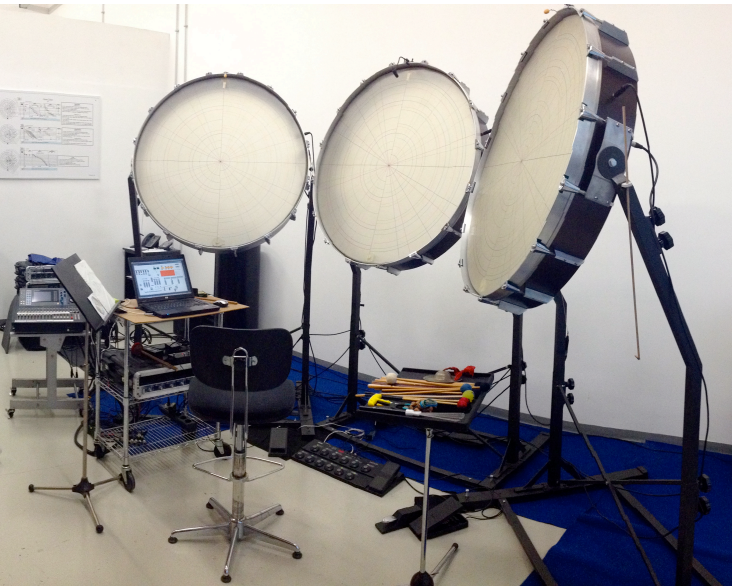
\includegraphics[width=0.99\columnwidth]{Graphics/foto/skin-act}
\caption[]{Michelangelo Lupone.\emph{Skin-Act}.}
\label{skinact}
\end{figure}

\section{Skin-Act}

In continuità con il \emph{Feed-drum}, gli \emph{Skin-Act} sono strumenti a percussione aumentati. In comune con hanno il fatto di avere una membrana di grancassa ma
mentre per il primo il feedback è generato tramite un altoparlante woofer posto
sotto la membrana, per gli \emph{Skin-Act} si ottiene tramite uno shaker applicato
sulla pelle stessa.

\begin{quote}
L’opera parte dall’idea di riprodurre lo spazio acustico, che è intorno
all’interprete, anche intorno all’ascoltatore, con caratteristiche coerenti di
mobilità e localizzazione. [\ldots]
Per realizzare una scrittura musicale che potesse evidenziare questa idea,
Lupone si è ispirato al concetto di spazio percepito e misurato attraverso il
tempo.[\ldots]

I ritmi e le durate rappresentano il materiale compositivo di base di
“Spazio curvo” sul quale vengono articolati i timbri eterogenei dello SkinAct.

L’opera è formalmente divisa in cinque sezioni, ognuna delle quali propone una
diversa concezione del ritmo:
\begin{enumerate}
  \item “nel suono” (battimenti ottenuti con le frequenze parziali della membrana),
  \item “nello spazio” (ritmi derivati dalla percezione dei movimenti e delle
localizzazioni dei suoni nello spazio acustico),
  \item“del suono” (ritmi ottenuti con tecniche di scomposizione temporale del
suono e ricomposizione a densità diverse),
  \item“con il suono” (ritmo organizzato con accenti e pause),
  \item“poliritmia” (ritmi diversi sovrapposti temporalmente).
\end{enumerate}

I tre \emph{Skin-Act} posti a distanza ravvicinata, si influenzano reciprocamente dando
luogo a una complessità elevata del fenomeno sonoro, e delle tecniche di
controllo.
\end{quote}

\begin{figure}%[t!]
\centering
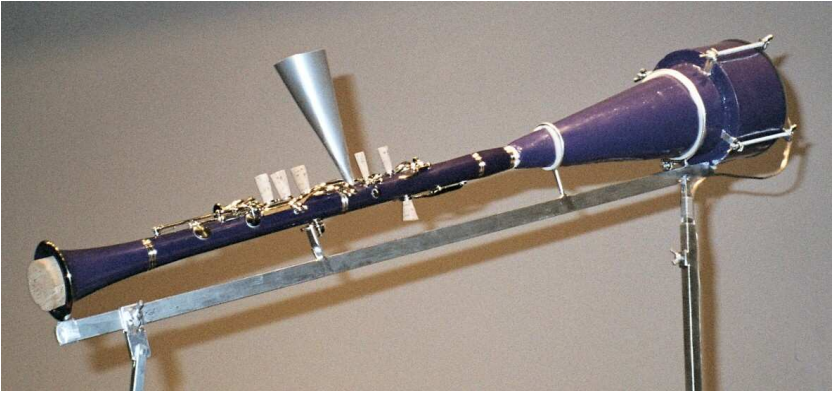
\includegraphics[width=0.99\columnwidth]{Graphics/foto/clarinetto_sospeso.PNG}
\caption[]{Silvia Lanzalone.\emph{Clarinetto Sospeso}.}
\label{clarinetto}
\end{figure}

\section{Il Clarinetto Sospeso}

Il \emph{Clarinetto Sospeso} è uno strumento aumentato costruito per il brano
\emph{Il Suono Incausato} (2005) da Silvia Lanzalone.

Questo strumento aumentato prevede l’uso del sughero con cui sono realizzati
sette tappi e tre leve: i tappi hanno lo scopo di chiudere i fori, le  leve
hanno lo scopo di tenere aperte o chiuse le chiavi. In partitura è indicato come
disporli.

Inoltre sono a disposizione dell’interprete quattro coni, uno di alluminio e tre
di cartone che vengono inseriti in determinate zone dello strumento per
amplificare l’irradiazione del suono. Completano lo strumento un cono di
piombo, scelto perché è un materiale acusticamente isolante ma non
fonoassorbente, inserito al posto del bocchino contenente un altoparlante e
un’asta di metallo su cui lo stesso strumento è fissato.

Durante l’esecuzione l’interprete è in grado di variare le sonorità emesse
dentro l’altoparlante operando manualmente om chiudendo manualmente le chiavi o
inserendo nei fori i tronchi di cono a sua disposizione.

\begin{quote}
Il \emph{Il Suono Incausato} propone una singolare installazione intorno al
clarinetto, in cui il rapporto con lo strumento non è più perseguito nella
tipica concatenazione logico-temporale per cui il suono (effetto) è ottenuto
tramite eccitazione della colonna d’aria presente nel tubo attraverso l’ancia
da parte dell’esecutore (causa). Il nuovo strumento, denominato
\emph{Clarinetto Sospeso}, è acusticamente autonomo poiché, anziché essere
“suonato” dall’interprete, viene da lui “esplorato” attraverso una serie di
interventi atti soprattutto a modificare le caratteristiche fisiche del tubo e
le combinazioni di fori aperti o chiusi, creando così nuove condizioni del
sistema vibrazionale. In questo brano il clarinetto è posto su di un sostegno
ed appare come sospeso, distante dallo strumentista, nonché fisicamente
modificato. [\ldots] Le manipolazioni effettuate sul \emph{Clarinetto Sospeso}, da
me definite “esplorazioni”, possono amplificare o attenuare alcune specifiche
risonanze, possono introdurre dei ritmi timbrici in sovrapposizione al suono di
base, possono agire per imitazione o per contrasto rispetto ad una particolare
modalità di articolazione del suono preesistente, possono non produrre alcun
effetto, coerentemente con le molteplici tipologie di connessione tra azione ed
evento. Le esplorazioni sono effettuate secondo un criterio di estemporaneità,
attraverso azioni che mettono in rilievo una componente gestuale e teatrale
dell’esecuzione.[\ldots]
Nessun suono può essere realmente \emph{Incausato} dal punto di vista fisico;
tuttavia nel \emph{Clarinetto Sospeso} i termini della relazione strumento/esecutore/suono
trovano una diversa relazione consequenziale.[…].d’arte
\end{quote}

\begin{figure}%[t!]
\centering
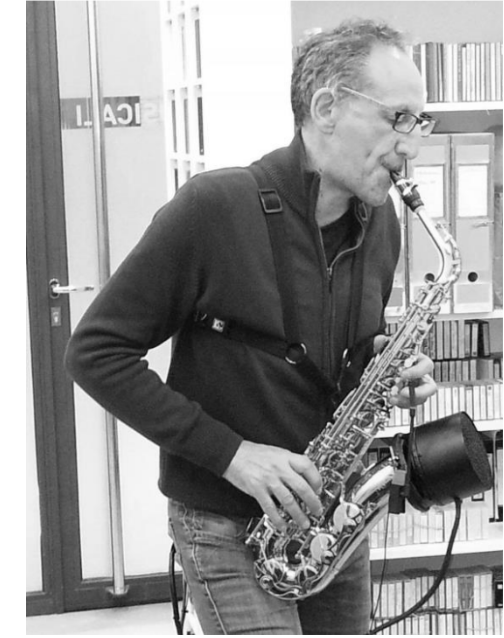
\includegraphics[width=0.99\columnwidth]{Graphics/foto/windback}
\caption[]{Enzo Filippetti.\emph{WindBack}.}
\label{windback}
\end{figure}

\section{Windback}

\emph{Windback} è uno strumento aumentato che usa il fenomeno del feedback
applicato a uno strumento a fiato.

Il primo \emph{Windback} è un prototipo ideato da Michelangelo Lupone per la sua
composizione \emph{In Sordina}. Lo strumento scelto è un sassofono a cui è stato applicato un microfono a metà del corpo e un altoparlante sulla campana.
Inoltre è contemplato anche l’uso di due pedali di controllo e un processore di
segnale.

Con questo prototipo è possibile ottenere:
\begin{enumerate}
  \item Suoni multifonici indipendenti
  \item Poliritmia
  \item Modificazione della struttura armonica
  \item Risonanza selettiva
\end{enumerate}

Questo prototipo è stato realizzato per l’opera musicale “In Sordina”.
Quest opera è stata composta utilizzando un sistema di risonanze acustiche del
sassofono caratterizzato da nuove modalità espressive.
Il flusso d’aria emesso dall’altoparlante, si propaga in senso contrario rispetto
al normale flusso d’aria prodotto da uno strumentista e genera un fenomeno di
feedback acustico in maniera potenzialmente infinita sostenendo sia la colonna
d’aria che il suono all’interno dello strumento.
Questo fenomeno permette l’esplorazione  del timbro del sassofono secondo
modalità non convenzionali e la scoperta dei dettagli del sistema di articolazione
del sassofono stesso.

\begin{figure}%[t!]
\centering
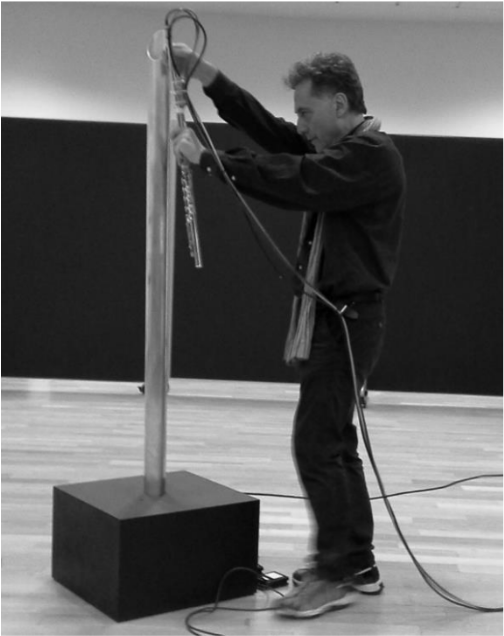
\includegraphics[width=0.99\columnwidth]{Graphics/foto/reso}
\caption[]{Gianni Trovalusci. \emph{ResoFlute}.}
\label{windback}
\end{figure}

\section{\emph{ResoFlute}}

\emph{ResoFlute} è un flauto traverso aumentato. Allo strumento tradizionale si sommano:

\begin{enumerate}
  \item due microfoni applicati internamente alla testata dello strumento al posto del
sughero tradizionale e cinque microfoni applicati esternamente.
  \item un sensore.
  \item comandi a pedale.
  \item un tubo in alluminio, di 10 cm di diametro e lungo 180 cm, per la diffusione e
la risonanza del suono.
\end{enumerate}

I cinque microfoni miniaturizzati sono fissati sul corpo dello strumento, accanto
ai fori delle chiavi, praticando dei fori nel tubo in base alla posizione di alcune chiavi. In questo modo è possibile rilevare le variazioni di pressione sonora riscontrabili nelle diverse parti del flauto.

Il corpo dello strumento è dotato di un sensore realizzato tramite una pellicola
piezo-elettrica, utilizzato per rilevare la posizione del pollice della mano
destra, che normalmente serve esclusivamente per tenere lo strumento. Un circuito
a soglia utilizza il segnale piezo-film  per produrre comandi on-off che
l'esecutore controlla in funzione della partitura.

Il suono dello strumento tradizionale è \emph{aumentato} anche attraverso l'uso
di un tubo di risonanza, che proietta il suono del flauto. Questo tubo in
alluminio è montato su di un contenitore in legno contenente un altoparlante.
L'altoparlante è collegato acusticamente al tubo attraverso un giunto conico, che aumenta l’efficacia della diffusione elettroacustica.

Tutti gli altri controlli di elaborazione del segnale vengono eseguiti tramite
pedali MIDI dotati di messaggi di variazioni di controllo e variazioni di programma.

Il flauto così \emph{aumentato} aggiunge possibilità timbriche allo strumento enfatizzando le caratteristiche di risonanza e diffusione spaziale del suono
attraverso il tubo risonante.

L'intero sistema comprende: l'algoritmo per la generazione di suoni sintetizzati
e l’elaborazione in tempo reale dei suoni del flauto. Il tutto è completato dal
fenomeno del feedback acustico.

Questo feedback dipende dalle caratteristiche del tubo risonante, responsabile
della diffusione del suono, e dalla posizione del flauto rispetto al tubo e ai microfoni interni.

L’equilibrio tra suono dello strumento ed elaborazioni elettroniche genera un
suono complesso a cui  vengono aggiunte integrazioni timbriche e diffusione
spaziale tramite la risonanza nel tubo di alluminio.
